%%%%%%%%%%%%%%%%%%%%%%%%%%%%%%%%%%%%%%%%%%%%%%%%%%%%%%%%%%%%%%%%%%%%%%%%%%%%%%%%
% experiment.tex: The CMS detector
%%%%%%%%%%%%%%%%%%%%%%%%%%%%%%%%%%%%%%%%%%%%%%%%%%%%%%%%%%%%%%%%%%%%%%%%%%%%%%%%
\chapter{The CMS Detector}
\label{sec:detector}
%%%%%%%%%%%%%%%%%%%%%%%%%%%%%%%%%%%%%%%%%%%%%%%%%%%%%%%%%%%%%%%%%%%%%%%%%%%%%%%%

The Compact Muon Solenoid (CMS) detector is one of two general-purpose detectors located at the large hadron collider (LHC) near Geneva, Switzerland. 
Within the 27 km ring of the LHC, two counter-rotating proton beams cross at several designated points, producing particle collisions with center-of-mass energies near \SI{13.7}{\tera\eV}. 
One of these crossing points is in the center of the CMS detector, where 'bunches' of $\thicksim10^{11}$ protons collide every \SI{25}{\nano\second} in a beam spot less than \SI{3}{\centi\meter} in length and \SI{20}{\micro\meter} in width. 
On average, each bunch crossing produces 32 proton-proton interactions, though most are 'pileup' interactions from soft QCD.

Occasionally, these collisions will produce exotic, high energy interactions between the quarks within the protons. 
Together, the primary and pileup interactions emit large numbers of secondary particles which radiate outward from the beam spot. 
The detector then measures and identifies these particles in order to reconstruct the physics processes that occurred during the collisions. 
While the bunches interact at a rate of \SI{40}{\mega\hertz}, the large amount of data produced in each collision and the limited data transfer and storage ability limits the final readout to $\thicksim$\SI{1}{\kilo\hertz}.

To successfully operate as a general purpose physics machine, the CMS detector must be able to rapidly identify outgoing particles from a large number of collisions, separate them into individual interactions, determine when physics processes of interest have occurred, record full event information in triggered events, and lastly accurately reconstruct final state particles in order to allow for detailed physics analysis. 

To fulfill the necessary timing, resolution, and particle identification requirements the CMS detector is split into several subsystems located concentrically around the collision point in a roughly cylindrical shape (\Cref{fig:detector}). 
Starting from the center, particles first pass through the pixel and strip trackers, which measure the position of charged particles to determine their vertex locations, trajectories, and momenta.
Next, particles enter the electromagnetic calorimeter (ECAL) which measures the energy of electrons, photons, and some mesons by completely stopping them through electromagnetic showers and measuring the resulting energy deposits.
After the ECAL, particles enter the hadronic calorimeter (HCAL), which measures neutral hadrons and other less-frequently-interacting particles which may pass through the ECAL. This is done by having many layers of dense absorber which induce hadronic showers, interleaved with scintillator layers to sample the resulting energy.
Finally, any remaining particles will pass into the muon chambers, which consist of cathode strips, resistive plates, and gas chambers which all track the motion of muons, as they are the only known particles visible to our detector which are unlikely to be stopped in the calorimeters.

In addition to the detecting subsystems, the central feature of the CMS detector is a superconducting solenoid located between the HCAL and muon chambers, which produces a \SI{3.8}{\tesla} magnetic field along the axis of the beam. 
A steel return yoke is located within the muon chambers to capture the fringe field from the solenoid, producing a field in the opposite direction to aid with the measurement of muon momenta.
The strong magnetic field provided by the solenoid reduces the necessary detector size to measure particle momentum and increases the precision of the measured \pt. 
The relatively small size of the resulting detector and use of the return yoke for muon measurements give the detector its name.

To best describe particle momenta and take advantage of the nearly cylindrical symmetry of the detector, a special coordinate system is defined. 
The Z-axis is chosen to be oriented along the beam line, and the transverse distance from it is referred to as $\rho$. 
Instead of the polar angle $\theta$, we use the pseudorapidity $\eta$,

\begin{equation}
    \label{eq:pseudo}
    \eta = - \log \left[\tan\left(\frac{\theta}{2}\right)\right]
\end{equation}

In special relativity, rapidity ($y$) is a measure of relativistic velocity with the feature that differences in rapidity are invariant under Lorentz transformations along the z-axis.
The definition of particle rapidity is shown in \Cref{eq:rapidity}, where E is the particle's total energy and p$_z$ is its z-momentum.

\begin{equation}
    \label{eq:rapidity}
    y = \frac{1}{2} ~\ln \left(\frac{E+p_z}{E-p_z}\right)
\end{equation}

Pseudorapidity is constructed to form an analogue of rapidity using only geometric information, and converges to match rapidity in the high-energy limit when particle mass is negligible.
Pseudorapidity is zero when perpendicular to the beam, and approaches positive and negative infinity along the z axis. 
Using this angular measure, selections using the angular separation of particles do not have strong dependence on longitudinal momentum and the overall distribution of outgoing collision products is nearly uniform in $\eta$ instead of strongly peaked towards zero and $\pi$ as it is in $\theta$.  
The angular distance in this coordinate system is defined as $\Delta R = \sqrt{(\eta_1-\eta_2)^2+(\phi_1-\phi_2)^2}$.

\begin{figure}[h]
    \includegraphics[width=\textwidth]{figures/cmsDetector.png}
    \centering
    \caption{The CMS detector.}
    \label{fig:detector}
\end{figure}

\section{Tracker}
The innermost part of the detector is the CMS tracker, which uses silicon detectors arranged in pixels and strips to measure ionization from charged products of the collision or their subsequent decays. 
A full description of this detector can be found in Reference \cite{trackerTDR}.
When ionizing particles pass through the silicon sensors, they excite electron-hole pairs within the silicon, which are collected via an applied electric field in the material and produce an output current pulse in the readout electronics.
The positions of these deposits in the silicon are then used to reconstruct the tracks of charged particles.
Using tracks, the charge and momentum of particles can be determined through their curvature in the magnetic field and particle trajectories can be extrapolated to the collision point in order to group tracks from the same interaction into vertices. 
High positional resolution is very important for track reconstruction to resolve individual vertices and separate pileup interactions as well as to precisely determine the track curvature over the length of the tracker. 

The pixel detectors are positioned in the inner part of the CMS tracker, where the high particle density requires the best position resolution. 
The pixel detector was upgraded in 2017 \cite{pixelUpgrade}, and the upgraded version is used in this description and all of the data samples in this analysis. 
The individual pixels are made of 100 $\times$ \SI{150}{\micro\meter} sensors which are placed in three disks in the endcap ($1.5<\lvert\eta\rvert<2.5$) region and four layers in the barrel ($\lvert\eta\rvert<1.5$) region, and have the short axis aligned in the $\phi$ direction so that measurements of curvature in $\phi$ from the magnetic field will have increased resolution from the smaller cell size. 
The resolution is further increased to sub-cell precision through charge-sharing from capacitive coupling in adjacent pixels, resulting in final position resolution on the order of \SI{10}{\micro\meter} along the short axis and \SI{20}{\micro\meter} in the longitudinal direction.

In deeper parts of the tracking system, the increased spatial dimension and reduced particle density reduces the need for pixel resolution and instead silicon strips of up to \SI{10}{\centi\meter} in length are used. 
In the barrel region, ten strip layers are present, reaching up to \SI{110}{\centi\meter} from the beam, and the strips are oriented slightly off-axis in alternating layers to increase the resolution in the z-direction. 
In the endcap, the strips are oriented perpendicularly to the beam in 12 disks up to a radial distance of \SI{270}{\centi\meter}.
Hits in the strip tracker have typical resolutions near \SI{200}{\micro\meter} in the Z-direction and \SI{20}{\micro\meter} in the $\phi$ direction.

The combination of pixel and strip trackers results in very good track reconstruction efficiency and position and momentum resolution.
Muon tracks are reconstructed with $>99\%$ efficiency over the entire $\eta$ range of the tracker, and vertices from multiple tracks originating at the same point are reconstructed with resolutions near \SI{50}{\micro\meter}.
Because higher energy tracks have less curvature, the \pt resolution of tracks decreases as the \pt itself increases. Tracks with typical \pt and $\eta$ used in this analysis (\pt near \SI{100}{\giga\eV} and $1.4<\eta<2.4$) have resolutions near 4$\%$. 

\begin{figure}[h]
    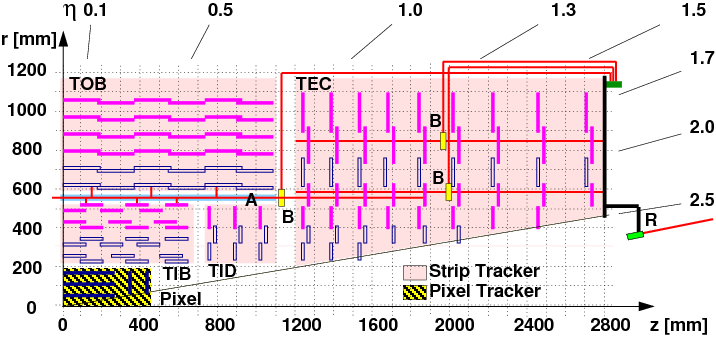
\includegraphics[width=\textwidth]{figures/cms_tracker.png}
    \centering
    \caption{A radial slice of the CMS Tracker.}
    \label{fig:cmsTracker}
\end{figure}


\section{ECAL}
The electromagnetic calorimeter sits outside of the tracker, and is split into a barrel and two endcap sections. 
The ECAL barrel covers $\lvert\eta\rvert<$1.479 and r$<$\SI{160}{\centi\meter}, while the endcaps cover 1.479$<\lvert\eta\rvert<$3 and $\lvert z \rvert<$\SI{4}{\meter}. 
Both sections consist of lead tungstate (PbWO$_4$) crystals, a dense (\SI{8.28}{\gram\per\cubic\centi\meter}) transparent crystal which produces scintillation light when it interacts with a high-energy particle. 
The scintillating radiation is absorbed by Avalanche Photo-diodes in the barrel and Vacuum Phototriodes in the endcaps to measure the energy deposited within each 
crystal. 

The crystals are tapered and arranged projectively at a slight angle to minimize inter-crystal gaps, pointing roughly \SI{3}{\degree} away from the collision point. 
They are about 23 cm, or 25 $X_0$, in depth, and have a transverse size of 2.2 $\times$ \SI{2.2}{\centi\meter^2} in the barrel and 2.9$\times$\SI{2.9}{\centi\meter^2} in the endcap. 
Each endcap is divided vertically into two 'Dees', each with 3660 crystals grouped into 5x5 units called 'Supercrystals'. 
During 2018 data taking, several supercrystals within the ECAL endcaps observed problems during data quality monitoring, and were 'masked' to remove their measurements from the total energy sums \Cref{fig:EEmasks}, removing roughly 2$\%$ of the total ECAL area.
Accurate measurements of ECAL deposits are necessary to reject potential backgrounds tracks with energy loss in ECAL.
To avoid potential backgrounds from tracks with missing energy from showers in these masked regions, signal tracks are required to have $\Delta R>0.1$ to any masked supercrystal.

\begin{figure}[h]
    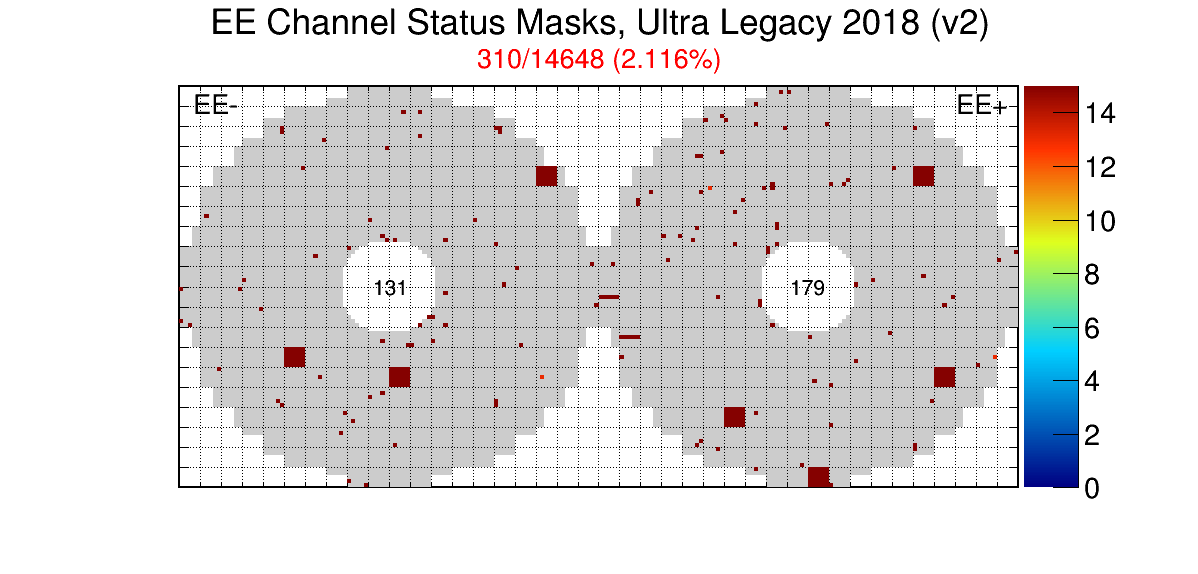
\includegraphics[width=\textwidth]{figures/EEChannelMasks.png}
    \centering
	\caption[Masked ECAL cells]{Transverse slices of the two ECAL endcaps showing the channel status for 2018 data taking. Active channels are in light gray, while inactive channels are colored dark red. The 3x3 squares of inactive tiles represent the inactive superclusters, with three in the negative $\eta$ endcap (left) and four in the positive $\eta$ endcap (right). In this view, the beam line is located at the center of the each ring, and the position of the cells from the middle of their respective center roughly corresponds to their position in r. \cite{EcalDPG}. While there are many individual inactive cells throughout both endcaps, no excess in background was observed outside of the inactive superclusters due to the diffuse nature of the electromagnetic showers in those events.}
    \label{fig:EEmasks}
\end{figure}

\section{HCAL}
The CMS hadronic calorimeter (HCAL) is a sampling calorimeter, which consists of alternating layers of brass absorber and plastic scintillator. 
Hadronic showers are primarily induced in the absorber, while the energy of the shower is sampled in each layer of scintillator and the sampled energy is used to estimate the total energy of the shower. 
While this sampling method lowers the precision of the energy measurement, it allows most of the detector material to be made of relatively cheap absorber instead of scintillating material, which results in a very substantial cost reduction due to the large amount of material required to stop high-energy hadrons.
The HCAL endcaps have 17 active layers of plastic scintillator and \SI{8}{\centi\meter} absorber, covering 1.4$<\eta<$2.4 and extending to $\lvert z \rvert<$ \SI{5.6}{\meter}, with a total radiation length near 200 X$_0$. 
The thickness of ECAL and HCAL is sufficient to stop nearly all mesons and hadrons produced in the collision, leaving only neutrinos, which are not visible in the detector, and muons. 
As the effective fixed target cross section for \dbrem is proportional to the thickness of the target, the large quantity of brass used in HCAL makes it the ideal location to produce potential signal events.
During data taking, the scintillation light from the sampling layers is collected in wavelength-shifting fibers then transported to readout electronics.
This light collection is done in the HCAL barrel (and Endcaps, prior to 2018) by hybrid photo-diodes (HPDs). 
Scintillation light from successive HPDs is summed together into 'towers' during readout, reducing the available depth information to one or two depths depending on location within the detector.

In the HCAL endcap (HE), radiation damage to the scintillating tiles caused by high particle flux necessitated the replacement of the avalanche photo-diodes with silicon photomultipliers (SiPMs) in 2018, which have three times better photon detection efficiency than HPDs.  
The SiPMs also have smaller footprints than the HPDs, allowing for more of them to be placed in the volume previously occupied by the HPDs and reducing the need for depth summation before readout. 
Using this, energy information from HE after the SiPM installation is now grouped into 6-7 depths as shown in \Cref{fig:HElayout}.

\begin{figure}[!htpb]
	   \centering
	      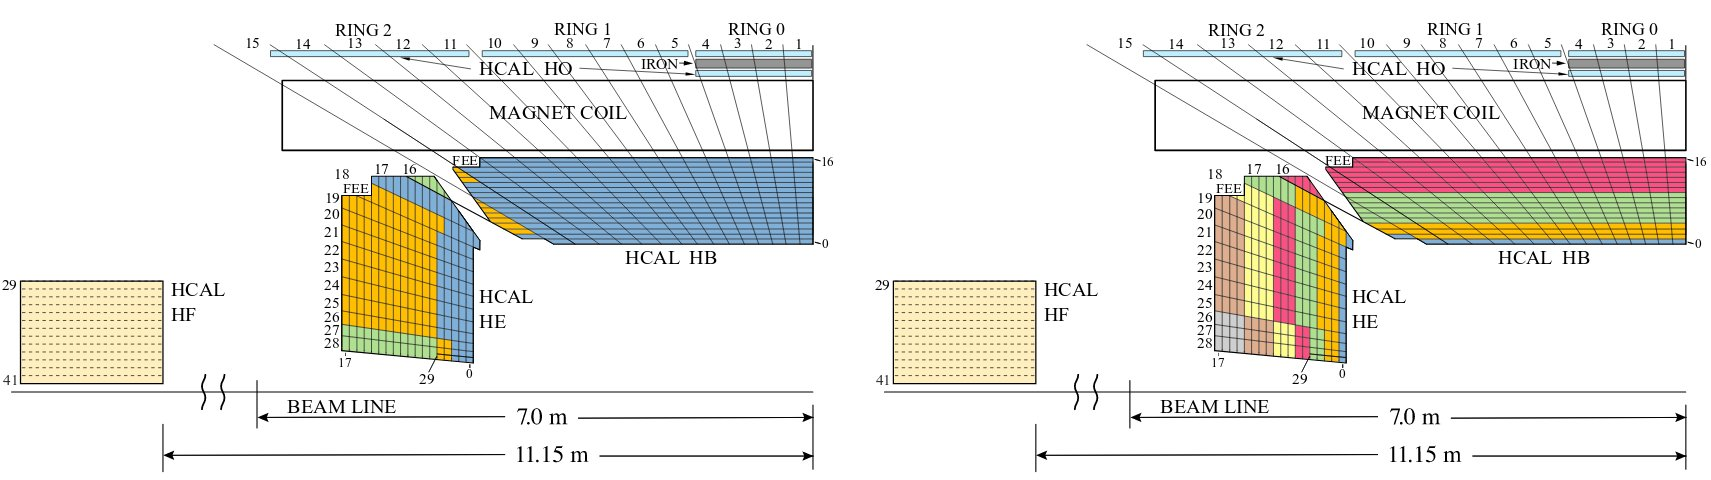
\includegraphics[width=\textwidth]{figures/HE_upgrade.jpg}
		 \caption[The 2018 HE upgrade]{The CMS HCAL geometry before (left) and after (right) the SiPM installation. Each rectangle represents a cell, and like-colored cells in HCAL at each i$\eta$ and i$\phi$ are summed to create a 'hit' at the depth represented by their color. These hits are the most granular HE information available. As the upgrade was only performed in HE for 2018 data taking, individual depth information is only available in the endcap for this analysis.}
	    \label{fig:HElayout}
\end{figure}

To reduce the data rate and the storage requirements, HCAL channels which fail to exceed set energy thresholds during data taking are not read out. 
This 'zero-suppression' is necessary for the detector to meet the strict timing requirements set by the number of collisions and the high frequency of the beam, but can distort the spectra of muon energy depositions by removing tails in the lower region of their energy depositions.
The increase in energy resolution from the SiPM upgrade greatly reduces this distortion by moving typical muon energy deposits further from the zero suppression threshold.
 
This improvement in muon energy resolution, in addition to the improved depth segmentation, provide very powerful tools for separating muon tracks from backgrounds as well as observing potential signal events.
Selected probe tracks for this analysis are thus required to be in the endcap, as the barrel regions do not have the resolution to effectively observe muons or reject missing energy from standard model processes or non-muon tracks.

In the readout chain, the HCAL sensors are grouped into 'sectors' containing clusters of cells. During the 2018 data taking two sectors could not be operated, resulting an a roughly 40 degree section with effectively no HCAL information. Similiarly to the inactive ECAL regions, these inoperable sectors could result in missing energy from showers within them, and so nearby tracks are excluded from the search. 
To avoid these regions, all probe tracks are required to be outside of the region of -3.0$<\eta<$ -1.3 and -1.57$<\phi<$-0.87, removing roughly 10$\%$ of potential tracks.

\section{Muon Systems}
After the tracker, ECAL, and HCAL, all standard model particles are expected to be absorbed except for muons and neutrinos, due to their small interaction cross sections.
While neutrinos are invisible to our detector, muons are electrically charged and so can deposit visible ionization when passing through a material.
To produce and capture this ionization and therefore identify and measure muons, muon chambers are placed outside of the solenoid which track muon trajectories using contained gases.
The measurement of muons is vital to this study, as precise muon measurements in the far reaches of the detector can look for energy loss with respect to the track, and muon detectors with very high efficiency can allow the identification of "missing" muons without major backgrounds from "missed" muons.

In the barrel region, $\lvert\eta\rvert<$1.2, drift tube (DT) detectors measure the position of passing high-energy muons. 
Each drift tube consists of a gas-filled metallic prism with an anode wire in the center and the metallic shell used as a cathode.
When muons produce ionization particles within the gas, a large applied voltage causes an avalanche effect which amplifies the number of electrons and ions which drift to the wires, then producing a measurable current.
The DT detectors are arranged in four 'stations' of increasing distance from the collision point, each containing several layers of 2.3$\times$\SI{4.2}{\centi\meter} cells, reaching up to a radial distance of \SI{7.5}{\meter}. 
The inner three stations have 8 layers of DT cells arranged perpendicularly to the beam axis and 4 layers parallel to it, while the outermost station only contains the perpendicular layers.
Each DT station is able to measure muon positions with longitudinal precision from 100 to \SI{300}{\micro\meter} and transverse precision from  60 to \SI{70}{\micro\meter}, allowing for precise measurements of muon \pt. 

In the endcaps, 0.9$<\lvert\eta\rvert<$2.4, cathode strip chambers (CSCs) are used instead of DTs due to the uneven magnetic field and increased radiation environment.
The CSCs operate on similar principles to the DTs, collecting ions and ionization electrons produced by muons passing through a contained gas. 
Instead of individual cells, each CSC layer uses anode wires stretched between cathode layers which are segmented into strips to provide positional information. 
By arranging the anode wires perpendicularly to the cathode strips, 2-D positional information can be measured by combining the cathode and anode location. 
Each CSC chamber consists of six layers, and four disks of two chambers each are located at staggered positions in the endcaps, shown in \Cref{fig:cscLayout}. 
The CSC chambers have similar resolution to the DTs, with the spatial resolution from each chamber ranging from 60 to \SI{120}{\micro\meter}.

In addition to the CSCs and DTs, the muon system contains resistive plate chambers (RPCs). 
Each DT chamber has one or two RPCs attached to it, and several CSCs have accompanying RPCs up to $\eta<$1.8. 
The RPCs follow the same gas ionization principles used in the CSCs and DTs, but use segmented metallic plates for both the anode and cathode.
The RPCs have much worse position resolution than the other two detectors, on the order of \SI{1}{\centi\meter}, but have an improved timing resolution of up to \SI{1}{\nano\second} to compliment the position measurements from the other systems.

\begin{figure}[h]
    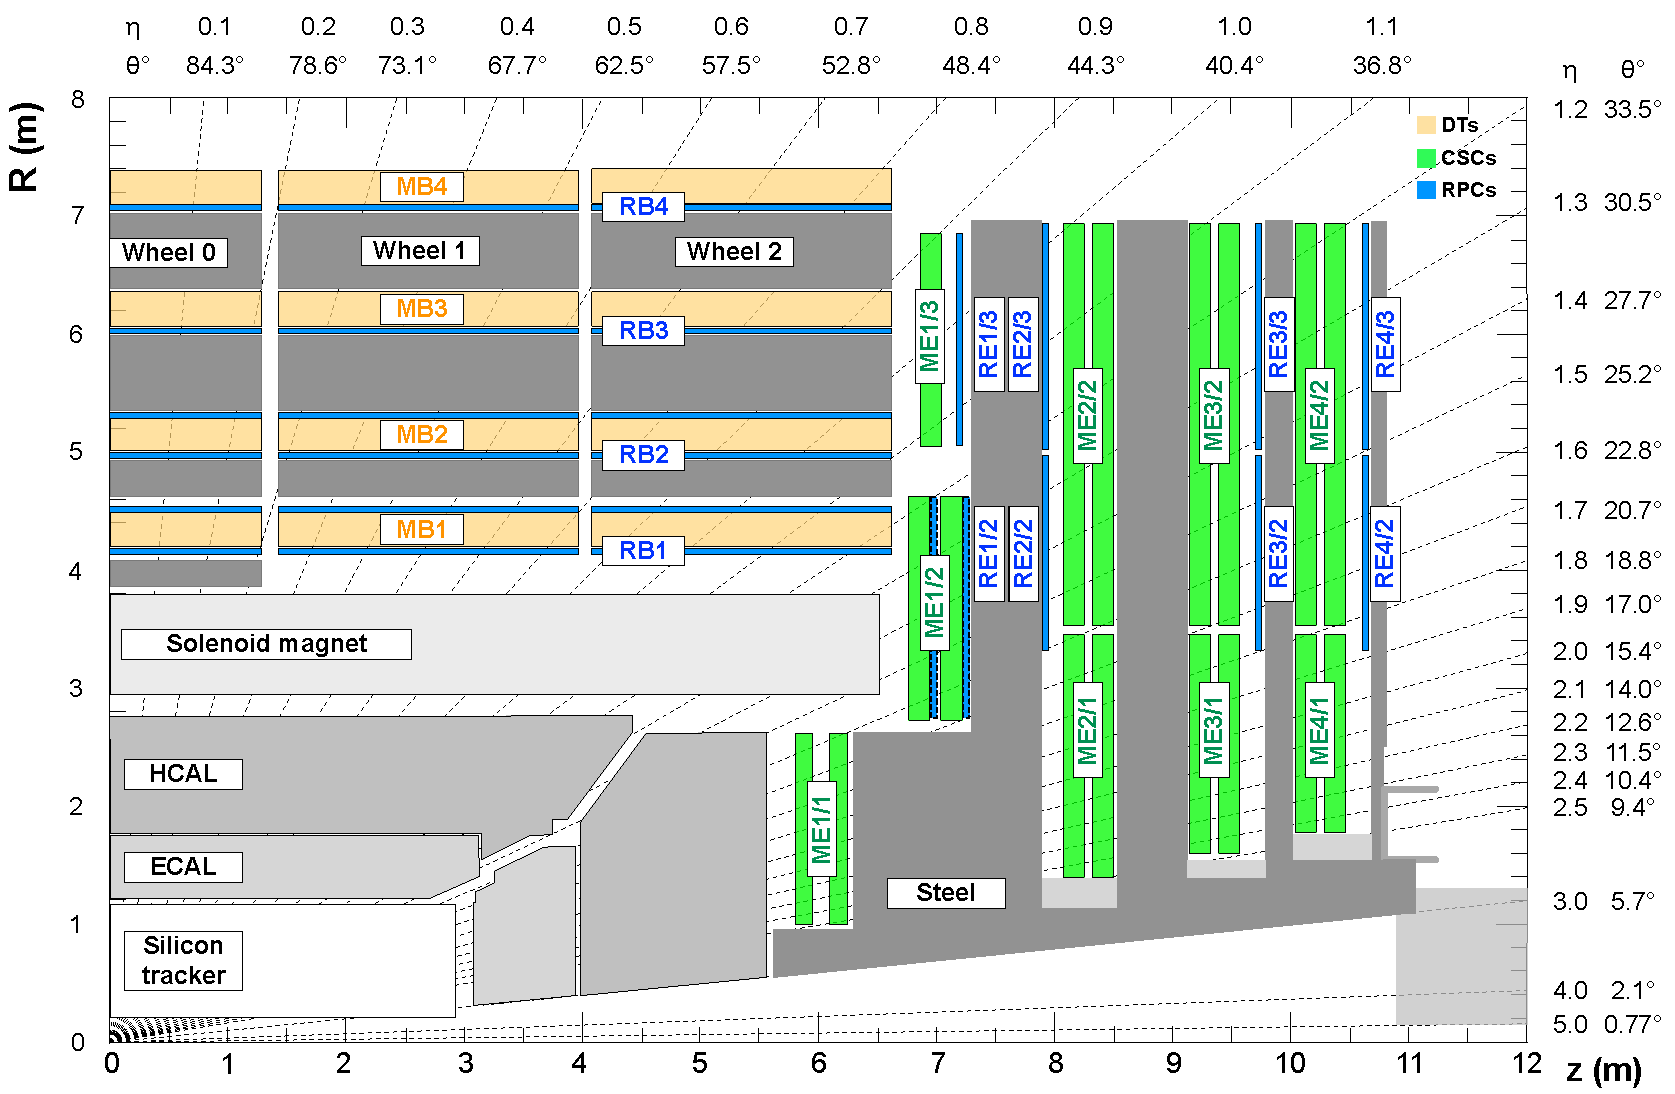
\includegraphics[width=\textwidth]{figures/cms_quadrant_run_ii.pdf}
    \centering
    \caption[Muon chamber layout in Run 2]{The muon chamber layout in one quadrant of CMS. The steel used for the return yoke is shown in dark gray, while the DTs, CSCs, and RPCs are shown in tan, green, and blue, respectively.}
    \label{fig:cscLayout}
\end{figure}


\section{Triggering}
The CMS trigger is performed using a two-stage approach. The first layer is the level one (L1) trigger, which uses limited event information to reduce the incoming event rate from \SI{40}{\mega\hertz} to about \SI{100}{\kilo\hertz} within \SI{2}{\pico\second}. 
Because of the high speed required, the L1 trigger uses dedicated hardware to make trigger decisions using simplified versions of the event reconstruction.
In the 2018 data set the L1 trigger uses only the muon chambers and calorimeters and includes no information from the tracker.
Clustering algorithms are used to reconstruct ECAL and HCAL to form electron, photon, jet, and hadronic $\tau$ candidates, while basic tracking algorithms are used to reconstruct muon candidates from hits in the muon chambers.
The L1 candidates in the event are then checked against existing selections for object kinematics and multiplicities, and events are chosen based on target physics of interest chosen by the CMS collaboration.

Events that pass the L1 trigger are then sent to the high-level trigger (HLT), which uses the full event information to make the more sophisticated final selections and reduce the event rate to near \SI{100}{\hertz}.
The increased calculation time allowed by the lower rate of events from the L1 trigger allows HLT to perform more complex object reconstruction and event selection than L1 using off-detector electronics, which calculated for L1 objects which match the requirements for HLT 'paths'.
Each path runs reconstruction and filtering steps for the specific objects and detector regions it defines.
For example, the isolated muon path (used in this analysis) reconstructs information from the muon systems and tracker near L1 muons which may pass the isolation and pt requirements of the path, stopping the calculation if the event fails the requirements at any point.
Events which fulfill all of the requirements of any HLT path are saved, and the event is stored for later reconstruction.

\section{Muon Reconstruction}
\label{sec:muonReco}
Muon reconstruction in CMS aims to convert event data of individual hits in the muon chambers and tracker into information about the underlying particle that produced those hits.
For the purposes of this search, tagging muons must be identified with very high purity to reduce background from fakes. 
Additionally, energy loss from signal events may appear as lowered energy in the reconstructed muons or interfere with their reconstruction such that it fails entirely, so detailed information about the reconstructed muons is used to identify potential signal events.
A full description of the muon reconstruction, as well as the resulting efficiency and resolution, can be seen in \cite{cmsMuonPerformance}.

First, hits from within a DT or CSC station are locally fit into tracks to form muon 'segments'.
The muon segments, along with any nearby RPC hits, are then fit together using a Kalman-Filter algorithm to form 'standalone' muons, which use only information from the muon chambers and the collision point.
Each standalone muon is then propagated back to the collision point through the magnetic field and detector material using estimates for the expected energy loss and track curvature.
The back-propagated muon is compared to each track from the silicon tracker in the event, and if a track is found with a similar trajectory the hits from the two candidates are combined into a global track.
An additional \kf algorithm is then used on the global track to make a global fit using the full information, creating a 'global' muon. 
In addition to the back-propagation, the tracking system tracks are extrapolated outward to the muon systems using the same assumptions, and any tracks which have at least one nearby muon segment are paired with those segments to form 'tracker' muons. 
When tracker, standalone, and global muons overlap, the candidate objects are combined into a single "particle flow" muon with separate references to the output of each reconstruction algorithm preserved.

In this work, we use both standalone and global muons. 
For the tagging muon, the high purity requirements make global muons the best choice of reconstruction algorithm. 
As no BSM processes should occur in the tag, the tracker information and muon segments should align, and the combination of the two gives the highest precision in momentum and location. 
For the probe muon, the large energy loss caused by \dbrem in the HCAL will introduce a mismatch between the muon chambers and the silicon tracker. 
Because of the increased position resolution in the pixel and strip trackers, the momentum of global muons favors the inner track information to the muon chambers in reconstruction.
As a result, if global muons are reconstructed in signal events the visible energy loss in the CSCs will be greatly reduced by this favoring of the tracker, and so the standalone muon reconstruction is used instead and compared with the selected track to look for potential energy differences.
